%\subsection{Suggestion Accuracy}
\subsection{Accuracy Comparison to $n$-gram, SLAMC, DNN, RNN~LMs in Code Completion}

%Comparison to $n$-gram

%DNN LM without Context

%DNN LM with Context

%\subsubsection{Comparison to $n$-gram, SLAMC, DNN, RNN~LMs}

%This section presents our comparative evaluation to the
%state-of-the-art {\em statistical LM approaches}. 
We compare {\tool} with the $n$-gram LM used in Hindle {\em et
  al.}~\cite{natural}, Deep Neural Network LM (DNN LM)~\cite{DNNLM12},
Recurrent Neural Network LM (RNN LM)~\cite{mikolov10,white-msr15} used
in White {\em et al.}~\cite{white-msr15}, and Nguyen {\em et al.}'s
SLAMC~\cite{fse13}.
%
Note that the original DNN LM~\cite{DNNLM12} works on texts and RNN
LM~\cite{mikolov10} was applied on only lexical code tokens by White
{\em et al.}~\cite{white-msr15}.
%
However, in the previous experiment, we have shown that adding
syntaxemes and sememes improves over using only lexemes for DNN LM.
Thus, in this experiment, for DNN LM and RNN LM, we used as input all
three sequences of lexemes, syntaxemes, and sememes.
% by concatenating their vectors.
%we operate it by treating all code tokens as texts.
SLAMC~\cite{fse13} is a LM that works on the $n$-grams of sememes and
lexemes to predict the next lexical token (no syntactic information is
used). It explores the pairs of tokens that often go together to
improve its accuracy as well. 
%
It also integrates LDA~\cite{lda} to derive the {\em topics} of the
current file via Bayesian inference into a $n$-gram topic
model~\cite{fse13}.
%
%It also integrates the {\em topics} of the current file in the model
%via Bayesian inference. That is, it integrates topic modeling with
%$n$-gram into~a~$n$-gram topic model~\cite{fse13}.
%
%We did not compare our model to the one by Tu {\em et
%  al.}~\cite{tu-fse14}, which improves over $n$-gram with caching of
%entities' names, since SLAMC was shown to outperform that model with
%caching. 
We did not compare {\tool} to Raychev {\em et al.}~\cite{ethz-pldi14}
and GraLan~\cite{icse15} since they operate only on API elements.

%This section presents another experiment that we conducted to compare
%{\tool}'s accuracy to that of the state-of-the-art approaches. We
%compare it to $n$-gram LM by Hindle {\em et al.}~\cite{natural}, Deep
%Neural Network LM (DNN LM) (see Section~2), and SLAMC~\cite{fse13},
%our prior work on semantic LM. Note that the original DNN LM works on
%texts. However, in our experiment, we operate it by treating all code
%tokens as texts. SLAMC~\cite{fse13} is a LM that works on the
%$n$-grams of sememes and lexemes to predict the next lexical token (no
%syntactic information is used). It also explores the pairs of tokens
%that often go together to improve its accuracy. Importantly, SLAMC
%integrates the {\em topics} of the current file in the model via
%Bayesian inference. That is, it integrates topic modeling with
%$n$-gram into~a~$n$-gram topic model~\cite{fse13}.  We did not compare
%our model to the one by Tu {\em et al.}~\cite{tu-fse14}, which
%improves over $n$-gram with caching of entities' names, because SLAMC
%was shown to outperform that model with caching. We did not compare
%{\tool} to Raychev {\em et al.}~\cite{ethz-pldi14} and
%GraLan~\cite{icse15} since they operate only on API elements.

% Table generated by Excel2LaTeX from sheet 'summary (2)'
\begin{table}[t]
  \centering
 \footnotesize
 \tabcolsep 4.4pt
 \renewcommand{\arraystretch}{0.9}
  \caption{Accuracy Comparison on All Projects}
  \begin{tabular}{l|l|l|l|l|l|l}
    \hline
    \textbf{Project} & \textbf{Top} & \textbf{$n$-gram} & \textbf{SLAMC} & \textbf{DNN LM} & \textbf{RNN LM} & \textbf{{\tool}} \\
    \hline
    ant   & 1     & 45.7\% & 49.5\% & 51.3\% & 52.1\% & 54.3\% \\
          & 2     & 57.1\% & 60.3\% & 67.4\% & 64.8\% & 70.6\% \\
          & 5     & 63.6\% & 65.8\% & 78.5\% & 78.4\% & 83.7\% \\
    \hline
    antlr & 1     & 50.0\% & 53.0\% & 54.0\% & 52.4\% & 57.4\% \\
          & 2     & 61.6\% & 65.1\% & 69.0\% & 62.7\% & 70.3\% \\
          & 5     & 68.7\% & 70.8\% & 81.9\% & 72.5\% & 83.5\% \\
    \hline
    batik & 1     & 55.8\% & 59.0\% & 59.4\% & 61.1\% & 64.8\% \\
          & 2     & 69.3\% & 70.2\% & 74.6\% & 73.2\% & 78.5\% \\
          & 5     & 73.5\% & 73.7\% & 84.3\% & 84.0\% & 88.2\% \\
    \hline
    cassandra & 1 & 44.9\% & 48.2\% & 48.7\% & 51.4\% & 54.7\% \\
          & 2     & 53.7\% & 57.4\% & 63.8\% & 64.0\% & 66.7\% \\
          & 5     & 61.2\% & 64.0\% & 78.9\% & 79.7\% & 80.3\% \\
    \hline
    db4o  & 1     & 34.0\% & 38.7\% & 42.3\% & 44.1\% & 49.2\% \\
          & 2     & 41.7\% & 46.6\% & 56.4\% & 57.4\% & 62.3\% \\
          & 5     & 47.5\% & 50.1\% & 73.2\% & 73.1\% & 77.6\% \\
    \hline
    itext & 1     & 45.3\% & 48.7\% & 49.0\% & 51.1\% & 55.3\% \\
          & 2     & 60.3\% & 64.1\% & 64.4\% & 61.4\% & 68.0\% \\
          & 5     & 69.3\% & 72.1\% & 79.7\% & 70.9\% & 82.6\% \\
    \hline
    jgit  & 1     & 46.0\% & 49.0\% & 49.0\% & 56.4\% & 53.8\% \\
          & 2     & 60.9\% & 63.6\% & 64.4\% & 65.4\% & 68.0\% \\
          & 5     & 70.6\% & 72.2\% & 79.6\% & 73.7\% & 82.6\% \\
    \hline
     lucene & 1    & 48.0\% & 52.2\% & 53.0\% & 53.4\% & 57.2\% \\
          & 2     & 60.6\% & 63.5\% & 68.9\% & 69.1\% & 73.0\% \\
          & 5     & 71.6\% & 73.6\% & 82.6\% & 82.9\% & 85.2\% \\
    \hline
    maven & 1     & 39.1\% & 43.4\% & 43.1\% & 44.7\% & 47.6\% \\
          & 2     & 49.0\% & 52.7\% & 58.7\% & 56.5\% & 62.8\% \\
          & 5     & 54.9\% & 58.4\% & 71.9\% & 67.9\% & 75.2\% \\
    \hline
    poi   & 1     & 38.6\% & 42.4\% & 44.8\% & 43.9\% & 49.3\% \\
          & 2     & 47.5\% & 51.4\% & 59.0\% & 52.9\% & 63.3\% \\
          & 5     & 55.6\% & 57.9\% & 73.2\% & 60.5\% & 77.4\% \\
    \hline
 \end{tabular}%
  \label{allaccuracytab}%
\end{table}%

% Table generated by Excel2LaTeX from sheet 'summary (2)'
%\begin{table}[t]
%  \centering
% \small
% \tabcolsep 3pt
% \renewcommand{\arraystretch}{0.9}
%  \caption{Accuracy Comparison on All Projects}
%  \begin{tabular}{l|l|l|l|l|l}
%    \hline
%    \textbf{Project} & \textbf{Top} & \textbf{$n$-gram} & \textbf{SLAMC} & \textbf{DNN LM} & \textbf{{\tool}} \\
%    \hline
%    ant   & 1     & 45.7\% & 49.5\% & 51.3\% & 54.3\% \\
%          & 2     & 57.1\% & 60.3\% & 67.4\% & 70.6\% \\
%          & 5     & 63.6\% & 65.8\% & 78.5\% & 83.7\% \\
%    \hline
%    antlr & 1     & 50.0\% & 53.0\% & 54.0\% & 57.4\% \\
%          & 2     & 61.6\% & 65.1\% & 69.0\% & 70.3\% \\
%          & 5     & 68.7\% & 70.8\% & 81.9\% & 83.5\% \\
%    \hline
%    batik & 1     & 55.8\% & 59.0\% & 59.4\% & 64.8\% \\
%          & 2     & 69.3\% & 70.2\% & 74.6\% & 78.5\% \\
%          & 5     & 73.5\% & 73.7\% & 84.3\% & 88.2\% \\
%    \hline
%    cassandra & 1     & 44.9\% & 48.2\% & 48.7\% & 54.7\% \\
%          & 2     & 53.7\% & 57.4\% & 63.8\% & 66.7\% \\
%          & 5     & 61.2\% & 64.0\% & 78.9\% & 80.3\% \\
%    \hline
%    db4o  & 1     & 34.0\% & 38.7\% & 42.3\% & 49.2\% \\
%          & 2     & 41.7\% & 46.6\% & 56.4\% & 62.3\% \\
%          & 5     & 47.5\% & 50.1\% & 73.2\% & 77.6\% \\
%    \hline
%    itext & 1     & 45.3\% & 48.7\% & 49.0\% & 55.3\% \\
%          & 2     & 60.3\% & 64.1\% & 64.4\% & 68.0\% \\
%          & 5     & 69.3\% & 72.1\% & 79.7\% & 82.6\% \\
%    \hline
%    jgit  & 1     & 46.0\% & 49.0\% & 49.0\% & 53.8\% \\
%          & 2     & 60.9\% & 63.6\% & 64.4\% & 68.0\% \\
%          & 5     & 70.6\% & 72.2\% & 79.6\% & 82.6\% \\
%    \hline
%    lucene & 1     & 48.0\% & 52.2\% & 53.0\% & 57.2\% \\
%          & 2     & 60.6\% & 63.5\% & 68.9\% & 73.0\% \\
%          & 5     & 71.6\% & 73.6\% & 82.6\% & 85.2\% \\
%    \hline
%    maven & 1     & 39.1\% & 43.4\% & 43.1\% & 47.6\% \\
%          & 2     & 49.0\% & 52.7\% & 58.7\% & 62.8\% \\
%          & 5     & 54.9\% & 58.4\% & 71.9\% & 75.2\% \\
%    \hline
%    poi   & 1     & 38.6\% & 42.4\% & 44.8\% & 49.3\% \\
%          & 2     & 47.5\% & 51.4\% & 59.0\% & 63.3\% \\
%          & 5     & 55.6\% & 57.9\% & 73.2\% & 77.4\% \\
%    \hline
% \end{tabular}%
%  \label{allaccuracytab}%
%\end{table}%

%% Table generated by Excel2LaTeX from sheet 'summary'
%\begin{table}[t]
%  \centering
%  \tabcolsep 3pt
%  \caption{Accuracy Comparison of Different Models}
%    \begin{tabular}{l|l|l|l|l|l}
%    \hline
%    \textbf{System} & \textbf{Top} & \textbf{\tool}* & \textbf{\tool} & \textbf{N-gram} & \textbf{SLAMC} & \textbf{SLAMC+Syn} \\
%    \hline
%    ant   & 1     & 51.3\% & 54.3\% & 45.7\% & 49.5\% & 51.3\% \\
%          & 2     & 67.4\% & 70.6\% & 57.1\% & 60.3\% & 62.5\% \\
%          & 5     & 78.5\% & 83.7\% & 63.6\% & 65.8\% & 67.9\% \\
%		\hline    			
%    antlr & 1     & 54.0\% & 57.4\% & 50.0\% & 53.0\% & 55.6\% \\
%          & 2     & 69.0\% & 70.3\% & 61.6\% & 65.1\% & 66.4\% \\
%          & 5     & 81.9\% & 83.5\% & 68.7\% & 70.8\% & 72.1\% \\
%		\hline
%    batik & 1     & 59.4\% & 64.8\% & 55.8\% & 59.0\% & 61.5\% \\
%          & 2     & 74.6\% & 78.5\% & 69.3\% & 70.2\% & 71.3\% \\
%          & 5     & 84.3\% & 88.2\% & 73.5\% & 73.7\% & 74.8\% \\
%		\hline			
%    cassandra & 1     & 48.7\% & 54.7\% & 44.9\% & 48.2\% & 50.8\% \\
%          & 2     & 63.8\% & 66.7\% & 53.7\% & 57.4\% & 59.1\% \\
%          & 5     & 78.9\% & 80.3\% & 61.2\% & 64.0\% & 65.3\% \\
%		\hline			
%    db4o  & 1     & 42.3\% & 48.8\% & 34.0\% & 38.7\% & 41.0\% \\
%          & 2     & 56.4\% & 61.5\% & 41.7\% & 46.6\% & 48.7\% \\
%          & 5     & 73.2\% & 76.9\% & 47.5\% & 50.1\% & 52.1\% \\
%		\hline			
%    itext & 1     & 49.0\% & 55.3\% & 45.3\% & 48.7\% & 52.5\% \\
%          & 2     & 64.4\% & 68.0\% & 60.3\% & 64.1\% & 66.6\% \\
%          & 5     & 79.7\% & 82.6\% & 69.3\% & 72.1\% & 73.7\% \\
%		\hline			
%    jgit  & 1     & 49.0\% & 53.8\% & 46.0\% & 49.0\% & 51.1\% \\
%          & 2     & 64.4\% & 68.0\% & 60.9\% & 63.6\% & 64.7\% \\
%          & 5     & 79.6\% & 82.6\% & 70.6\% & 72.2\% & 73.3\% \\
%		\hline			
%    lucene & 1     & 53.0\% & 57.2\% & 48.0\% & 52.2\% & 54.4\% \\
%          & 2     & 68.9\% & 73.0\% & 62.6\% & 63.5\% & 65.6\% \\
%          & 5     & 82.6\% & 85.2\% & 71.6\% & 73.6\% & 75.5\% \\
%		\hline			
%    maven & 1     & 43.1\% & 47.6\% & 39.1\% & 43.4\% & 45.0\% \\
%          & 2     & 58.7\% & 62.8\% & 49.0\% & 52.7\% & 54.3\% \\
%          & 5     & 71.9\% & 75.2\% & 54.9\% & 58.4\% & 60.0\% \\
%		\hline			
%    poi   & 1     & 44.8\% & 49.3\% & 38.6\% & 42.4\% & 44.3\% \\
%          & 2     & 59.0\% & 63.3\% & 47.5\% & 51.4\% & 53.4\% \\
%          & 5     & 73.2\% & 77.4\% & 55.6\% & 57.9\% & 59.4\% \\
%    \hline
%    \end{tabular}%
%  \label{allaccuracytab}%
%\end{table}%


\begin{figure}[t]
\centering
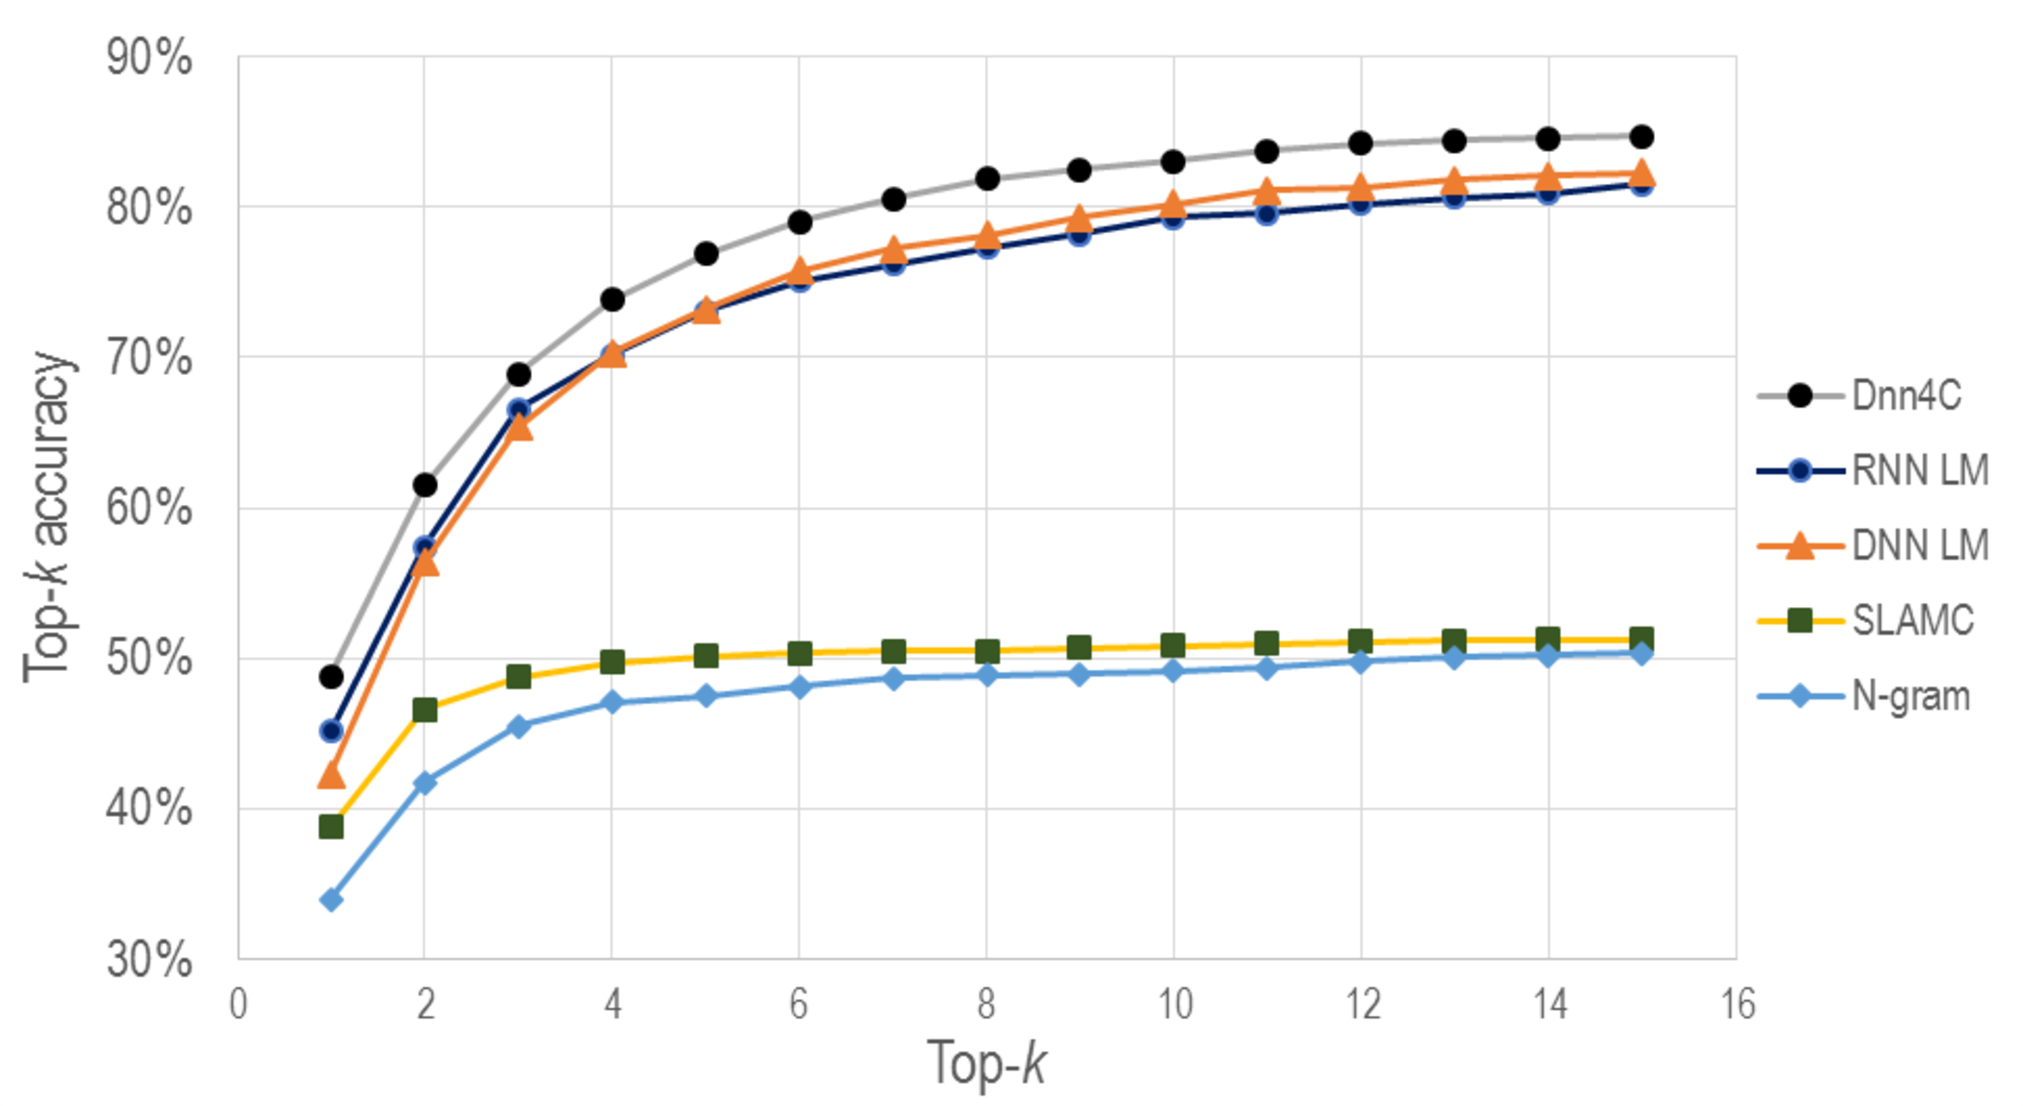
\includegraphics[width=3.5in]{db4o-new-3.pdf} %db4o-new-2.pdf {0.5 db4o.pdf, 0.46 sensitivity_approaches.pdf}
\vspace{-0.05in}
\caption{Top-$k$ Accuracy of Different Approaches on Db4o}
\label{approachesfig}
\end{figure}

%
%In general, {\tool} achieves higher accuracy than other approaches
%including DNN LM. {\tool} and DNN LM, which are based on DNN, achieve
%much higher accuracy than others in the larger values of top rank $k$,
%and reasonably higher accuracy in the smaller values of $k$.
%

Fig.~\ref{approachesfig} shows the comparison on \code{Db4o}
project for top-$k$~accuracy, $k$ = 1--15.  As seen,
{\tool} achieves higher~accuracy than the other approaches. At top-1
accuracy, {\tool} has relative improvements of {\bf 11.6\%}, {\bf
  16.3\%, 27.1\%}, and {\bf 44.7\%} over RNN LM, DNN LM, SLAMC, and
$n$-gram models, respectively. 
%
%At top-5 accuracy, such improvements are {\bf 6.2\%}, {\bf 6\%}, {\bf
%  54.9\%}, and {\bf 63.4\%}.
%
The three NN-based models achieve higher accuracy than the two
$n$-gram-based ones.
%, SLAMC and $n$-gram LM. 
%
%Such comparison was reported for texts in NLP~\cite{dnnbook}.
%
%This result confirms such comparison for source code. 
Among the NN-based models, with the same three features, {\tool}
outperforms RNN LM and DNN LM~relatively {\bf 11.6\%} and {\bf 16.3\%}
at top-1 accuracy. The absolute improvement percentages are reported
in Table~\ref{allaccuracytab}.
At a higher top rank $k$ from 10--15, {\tool} has much higher accuracy
than $n$-gram ({\bf 68.9\%} relatively) and SLAMC ({\bf 66.0\%}), and
higher than both RNN and DNN LMs.

% ({\bf 3.5\%}, {\bf 3.8\%}).

%Moreover, {\tool} outperforms DNN LM from 2.8--15.3\% for all top
%ranks $k$.

Table~\ref{allaccuracytab} shows the comparison result for {\em all
  projects}. At top-1 accuracy, {\tool} achieves relative improvements
from {\bf 14.8--44.7\%} over $n$-gram, {\bf 8.3--27.1\%} over SLAMC,
{\bf 5.9--16.3\%} over DNN LM, and {\bf 5.6--11.6\%} over RNN LM.

% ICSE'16
%If the models would suggest 5 candidates for the next token, {\tool}
%achieves relatively higher accuracy from {\bf 17.0--61.9\%} over
%$n$-gram model, from {\bf 14.4--53.5\%} over SLAMC, and from {\bf
%  1.8--6.7\%} over DNN LM. 
%


% in code suggestion than DNN LM, SLAMC, and $n$-gram models.


%Table {\ref{allaccuracytab}} shows the accuracy of our approach compared with other approaches. Column {\textbf{\tool}} is corresponding to our approach. Column {\textbf{\tool}*} is the accuracy of our tool without consideration of syntactic and semantic information.  Column {\textbf{N-gram}} is for N-gram approach,  column {\textbf{SLAMC}} is for SLAMC model modified to recommend lexeme and column {\textbf{SLAMC+Syn}} is the accuracy with SLAMC model extended with syntactic features.

%Implication:

%Tien
%1. {\textbf{\tool}} always achieve the best results in comparison with
%other approaches. {\textbf{\tool}*} achieve better results than
%{\textbf{N-gram}} and {\textbf{SLAMC}}. Its accuracy is comparable to
%{\textbf{SLAMC+Syn}} at low $k$ ( in $top-k$) but better than
%{\textbf{SLAMC+Syn}} at high $k$. {\textbf{SLAMC+Syn}} achieve better
%accuracy than {\textbf{N-gram}} and {\textbf{SLAMC}} but less accuracy
%than {\textbf{\tool}}.

%2. In details, at $top-1$, {\textbf{\tool}*} has better accuracy than
%{\textbf{N-gram}} from 3.0\% to 8.3\% (6.5\% to 24.4\% relatively).
%It improves over {\textbf{SLAMC}} from 0.0\% to 3.6\% (0.0\% to 9.3\%
%relatively). In some cases, {\textbf{\tool}*}'s accuracy is higher
%than {\textbf{SLAMC+Syn}} and in other cases, it is not. However, the
%difference is not significant.  {\textbf{\tool}} improves over
%{\textbf{N-gram}} from 7.4\% to 14.8\% (14.8\% to 43.5\% relatively).
%It improves over {\textbf{SLAMC+Syn}} from 1.8\% to 7.8\% (3.2\% to
%19.0\% relatively).


%3. At $top-5$, {\textbf{\tool}*} has better accuracy than
%{\textbf{N-gram}} from 9.0\% to 25.7\% (12.7\% to 54.1\% relatively).
%It improves over {\textbf{SLAMC}} from 7.4\% to 23.1\% (10.2\% to
%46.1\% relatively). It also improves over {\textbf{SLAMC+Syn}} from
%6.0\% to 21.1\% (8.1\% to 40.5\% relatively).  {\textbf{\tool}}
%improves over {\textbf{N-gram}} from 12.0\% to 29.4\% (17.0\% to
%61.9\% relatively).  {\textbf{\tool}} improves over
%{\textbf{SLAMC+Syn}} from 8.9\% to 24.8\% (12.1\% to 47.6\%
%relatively).  We checked the reason that {\textbf{\tool}} and
%{\textbf{\tool}*} have much improvement at high $top-k$. We saw that
%{\textbf{N-gram}}, {\textbf{SLAMC}} and {\textbf{SLAMC+Syn}} cannot
%predict $n-gram$ if that $n-gram$ has never appeared which leads to
%the $top-k$ accuracy get flat at high $k$. In other way,
%{\textbf{\tool}*} and {\textbf{\tool}} can predict event $n-gram$
%which has never appeared due to the mechanism of similar context in
%DNN language model.

%\[MRR({T_{test}},{T_{pred}}) = \frac{1}{{|{T_{test}}|}}\sum\limits_{i = 1}^{|{T_{test}}|} {\frac{1}{{index_i}}} \]

% Table generated by Excel2LaTeX from sheet 'summary'
\begin{table}[t]
  \centering
  \small
  \tabcolsep 3pt 
  \renewcommand{\arraystretch}{0.7}
  \caption{Mean Reciprocal Rank (MRR) Comparison}
    \begin{tabular}{l|l|l|l|l|l}
    \hline
    \textbf{Project} & {\textbf{$N$-gram}} & {\textbf{SLAMC}} & \textbf{DNN LM} & {\bf RNN LM} & \textbf{{\tool}} \\
    \hline
    ant   & 0.537 & 0.568 & 0.639 &     0.639   & 0.662 \\
    antlr & 0.584 & 0.616 & 0.662 &     0.628   & 0.695 \\
    batik & 0.640 & 0.674 & 0.706 &     0.719   & 0.737 \\
    cassandra & 0.519 & 0.555 & 0.616 & 0.638   & 0.656 \\
    db4o  & 0.400 & 0.439 & 0.581 &     0.586   & 0.611 \\
    itext & 0.577 & 0.617 & 0.625 &     0.601   & 0.656 \\
    jgit  & 0.588 & 0.619 & 0.673 &     0.647   & 0.701 \\
    lucene & 0.599 & 0.631 & 0.689 &    0.681   & 0.713 \\
    maven & 0.463 & 0.524 & 0.558 &     0.553   & 0.578 \\
    poi   & 0.459 & 0.492 &  0.563 &    0.516  & 0.583 \\
    \hline
    \end{tabular}
  \label{mrrtab}%
\end{table}%

% Table generated by Excel2LaTeX from sheet 'summary'
%\begin{table}[t]
%  \centering
%	\tabcolsep 3pt 
%  \renewcommand{\arraystretch}{0.7}
%  \caption{Mean Reciprocal Rank (MRR) Comparison}
%    \begin{tabular}{l|l|l|l|l}
%    \hline
%    \textbf{Project} & {\textbf{$N$-gram}} & {\textbf{SLAMC}} & \textbf{DNN LM} & \textbf{{\tool}} \\
%    \hline
%    ant   & 0.537 & 0.568 & 0.639 & 0.662 \\
%    antlr & 0.584 & 0.616 & 0.662 & 0.695 \\
%    batik & 0.640 & 0.674 & 0.706 & 0.737 \\
%    cassandra & 0.519 & 0.555 & 0.616 & 0.656 \\
%    db4o  & 0.400 & 0.439 & 0.581 & 0.611 \\
%    itext & 0.577 & 0.617 & 0.625 & 0.656 \\
%    jgit  & 0.588 & 0.619 & 0.673 & 0.701 \\
%    lucene & 0.599 & 0.631 & 0.689 & 0.713 \\
%    maven & 0.463 & 0.524 & 0.558 & 0.578 \\
%    poi   & 0.459 & 0.492 &  0.563 & 0.583 \\
%    \hline
%    \end{tabular}
%  \label{mrrtab}%
%\end{table}%


\vspace{0.03in}
\noindent {\bf Mean Reciprocal Rank (MRR).} We also
measured Mean Reciprocal Rank (MRR) to evaluate the models based on the
ranked list of suggested tokens.
%
The MRR value is computed as the average of the reciprocal ranks of
results for a set of suggestion cases:
\indent $MRR = \frac{1}{{|{T_{test}}|}}\sum\limits_{i = 1}^{|{T_{test}}|} {\frac{1}{{index_i}}} $
where $index_i$ is the index of the actual token in the
resulting ranked list at the $i$-th suggestion, and $|T_{test}|$ is
the number of suggestion cases.
%
%where $T_{test}$ is the true next tokens in the testing set for
%suggestion; $index_i$ is the index in the ranked list of predicted
%token at a suggestion, where the true next token is retrieved for the
%$i$-th query in the testing set. 
The closer to 1 the MRR value, the better the ranking of a model. 

As seen in Table~\ref{mrrtab}, {\tool} can achieve the highest MRR of
0.737, meaning that {\em on average in 2 suggestion cases, it can
  correctly rank the actual token as the top candidate in one case and
  at the second place in the resulting list in the other case}. For
all projects, MRR is 0.66 on average. That is, {\em among 3 cases, it
  would rank the actual token at the second place in two cases, and
  likely rank the actual token as the top candidate in the other
  case}.

In comparison, {\tool} improves MRR,
% relatively over the $n$-gram model up to {\bf 52.6\%}, over SLAMC up
% to {\bf 39.1\%}, over DNN LM up to {\bf 6.4\%}, and over RNN LM up
% to {\bf 13.0\%}.
\ie for a suggestion, the actual next token is generally ranked
higher in {\tool}'s resulting list than in the resulting lists of
other approaches.

%%In brief, {\em {\tool} consistently achieves better accuracy than others}.

%In comparison, {\tool} improves MRR accuracy relatively over the
%$n$-gram model from {\bf 13.7--52.6\%}, the SLAMC model from {\bf
%  9.3--39.1\%}, the DNN LM from {\bf 3.5--6.4\%}, the RNN LM from {\bf
%  2.7--5.5\%}.
%---------------------------

%This result is consistent with the comparison using top-$k$ accuracy.

%Moreover, in the subject project \code{batik}, with the MRR of {\bf
%  0.737}, every time that {\tool} has ranked the actual next token at
%the second place in its resulting list, it would likely rank the
%actual token as the top candidate for the next suggestion. On average,
%after every two times of ranking for the actual token at the second
%place, {\tool} would rank the actual token at the top.

%-------
%As seen in Table~\ref{mrrtab}, {\tool} improves MRR accuracy
%relatively over the $n$-gram model from {\bf 13.7--52.6\%}, the SLAMC
%model from {\bf 9.3--39.1\%}, and the DNN LM from {\bf 3.5--6.4\%}.
%
%That is, for a suggestion, the actual next token is generally ranked
%higher in {\tool}'s resulting list than the resulting lists of other
%models.  This result is consistent with the comparison using
%top-$k$ accuracy.
%
%Moreover, in the subject project \code{batik}, with the MRR of {\bf
%  0.737}, every time that {\tool} has ranked the actual next token at
%the second place in its resulting list, it would likely rank the
%actual token as the top candidate for the next suggestion. On average,
%after every two times of ranking for the actual token at the second
%place, {\tool} would rank the actual token at the top.
%------

%That is, with its suggestion list, {\tool} achieves higher accuracy in
%suggesting the next token.


%Those ranked lists of links $L_{pred}$ are used to evaluate a goal
%function \code{MAP($G_{test}, L_{pred}$)}, which is used to find the
%optimized value of $\alpha_1$.
%The $\alpha_1$ value corresponding to the highest value for \code{MAP}
%will be returned. The goal function $MAP$ in our algorithm is the mean
%average precision as proposed in {\cite{sun-ase11}}.










%4. To see if there are significant improvement over different approach, We then use t-test (with confidence of 0.95) over the $top-k$ accuracy to check the significance of hypotheses that an approach has more significant improvement over other approach. A hypothesis is considered significant if checking $p-value$ is smaller than 0.005.
%% Table generated by Excel2LaTeX from sheet 'summary'
%\begin{table}[h]
  %\small
	%\tabcolsep 1pt
  %\centering
    %\begin{tabular}{l|l|l|l|l}
    %\hline
           %&{\textbf{N-gram}}<{\textbf{SLAMC}} & {\textbf{SLAMC}}<{\textbf{SLAMC+Syn}} & {\textbf{SLAMC+Syn}}<{\textbf{\tool}} & {\textbf{\tool}}<{\textbf{\tool}*} \\
    %\hline
    %p-value&$10^{-14}$     & $10^{-16}$          & $0.0005$         & $10^{-15}$ \\
    %\hline
    %\end{tabular}%
  %\label{testingtab}%
  %\caption{Testing Significant Improvement between Approaches}
%\end{table}%
%
%Table {\ref{testingtab}} shows that our approaches are better than approaches based on {\textbf{SLAMC}}, which in turn better than {\textbf{N-gram}} approach.
%
%\subsection{Case Studies}


%%%% REMOVED
%\input{bayesmodel}
